\documentclass[a4paper,12pt,english]{article}
 
\usepackage[utf8]{inputenc}
\usepackage[T1]{fontenc}
\usepackage{babel}

\usepackage{hyperref}
\def\UrlBreaks{\do\/\do-}
\usepackage{graphicx}
\usepackage{wrapfig}
\usepackage[table,xcdraw]{xcolor}

\usepackage[inline]{enumitem} % inline lists
\usepackage{caption}
\usepackage{subcaption}
\usepackage{float}
\newcommand{\infra}{\emph{infra}}
\newcommand{\TODO}{\fbox{\textcolor{red}{TODO}}}

\begin{document}

\begin{titlepage}
	\centering
	\fbox{\begin{minipage}{\textwidth}
	\centering
	\vspace{0.3cm}
    {\scshape\LARGE\bfseries Project Report\par}
	\vspace{0.2cm}
	{\Large\bfseries Automated Essay Scoring \par}
	\vspace{0.3cm}
    \end{minipage}}
	
	\vfill
	
\includegraphics[width=0.5\textwidth]{fig/psl.jpg}\par\vspace{0cm}
	{\scshape\Large IASD Master \par}
	\vfill
	{\Large Pierre-François \textsc{Massiani}\par}
	{\Large Guillaume \textsc{Le Moing}\par}
	\vfill
	work completed during the\par
	Natural Language Processing class
	\vfill
    {\large April 25\textsuperscript{th}  , 2020\par}
\end{titlepage}
\tableofcontents
\newpage

\section{Introduction}

This is the final project for the « Natural Language Processing » class of Master IASD (Artificial Intelligence, Systems, Data), a joint PSL University Master program hosted by Paris-Dauphine, École normale supérieure, and MINES ParisTech.

In this project we propose and compare different neural network architectures as well as learning strategies for the automated essay scoring task.
We test our algorithms using the data from the ASAP competition on Kaggle~\cite{kaggle} sponsored by The Hewlett Foundation.

Our project was implemented in Python. The code is available on a Github repository at this address:
\begin{center}
	\url{https://github.com/16lemoing/automated-essay-scoring/} 
\end{center}
Instructions are included in the repository to run the code on your machine.

\subsection{The automated essay scoring task}
\TODO{décrire succintement la tâche à accomplir : on donnera les détails dans la partie dataset}

\subsection{Related work}
\TODO{citer 4,5 travaux qui ont été publiés là dessus}
%par ex
%https://cs224d.stanford.edu/reports/huyenn.pdf
%https://pdfs.semanticscholar.org/21d8/22e9f0783d79ab19563d36c006f202b508e0.pdf
%http://cs229.stanford.edu/proj2013/SongZhao-AutomatedEssayScoring.pdf
%https://github.com/Turanga1/Automated-Essay-Scoring/blob/master/Automatic%20Student%20Essay%20Assessment.pdf
%https://github.com/m-chanakya/AutoEssayGrading/blob/master/papers/paper1.pdf

\section{A Neural Network based approach}

We choose to rely on neural networks for this task.
We describe in this section the whole pipeline from raw essays to the prediction of the scores.
For each part, we present different options that are included in this project.

\subsection{Words embedding}
Essays have to be turned into vectors of numbers before being fed to a neural network.
One popular strategy is to assign a vector to every single word in the text.
The required dimension for the vectors depends on the richness of the vocabulary (both in quantity and lexical diversity).
\subsubsection{Random}
This is the most basic embedding.
We assign to each word of the vocabulary a vector of random samples from a normal (Gaussian) distribution.
\subsubsection{Word2Vec}
We propose to train a Word2Vec model~\cite{mikolov2013efficient} on the sentences extracted from the training essays.
This model learns meaningful embeddings by trying to guess a word from its context (a few words before and after in the sentence).
To do this each word of the context is turned into a vector from which the prediction is made.
Those vectors are what we use as embeddings once the model is trained.
Each set of essays deals with a different topic.
We hope to capture topic-related knowledge from the corpora by learning the embedding directly from the set of training essays.
\subsubsection{GloVe}
We also propose a different strategy for getting word embeddings using GloVe~\cite{pennington2014glove}.
The particularity of GloVe embedding is that there are linear substructures between words sharing semantic aspects.
For this embedding, we decide not to train the GloVe model from scratch but use a pre-trained model on large-scale corpora such as Wikipedia instead.

\subsection{Essay preprocessing}
We present here a few preprocessing methods that can help the learning process.
\subsubsection{Spelling errors correction}
Reading a few essays, we realised that there were lots of misspelled words in the essays.
This can impair the prediction performance because we cannot provide a meaningful embedding to misspelled words and we have a much larger vocabulary.
It would have come in handy to have a python wrapper for a correction tool such as LanguageTool which handles both syntaxic and grammatical errors.
Instead we used pyspellchecker package which gives a list of the most plausible correction candidates for each of the misspelled words (but do not consider the sentence as a whole).
\subsubsection{Stopwords removal}
There are some very common words, called stopwords that usually do not add much meaning to the sentence.
A common preprocessing step in natural language processing consists in removing these words that can pollute the learning process.
However, in our case it is unclear whether we should remove these words or not.
For example we need to take them into account when evaluating the gramatical correctness of a sentence.
That being said, it would be surprising that our model learns what is a grammaticaly correct sentence from such a small corpus.

\subsection{Essay processing}
We describe here how the essays are transformed so that they can be understood by a neural network.
\subsubsection{Word tokenization}
The first step is to transform essays into tokens (isolated words).
To do that we transform every special character into a space symbol and then split the essay at every occurence of the space symbol.
\subsubsection{Essay padded encoding}
Then we assign to each word its index in the vocabulary. This index will be used as a key when retrieving the word embedding.
To enable batch-learning we pad every essay so that it matches the length of the longest essay.

\subsection{Multitask model}
The dataset contains multiple essay tasks which are scored on different scales.
This makes it difficult to learn all tasks jointly.
However this can be addressed by normalizing the scores.
\subsubsection{Score normalization}
We rescale all the scores so that they fall into $[0,1]$, by applying this simple linear transformation:
\begin{equation}
s_{norm} = (s - s_{min}) / (s_{max} - s_{min})
\end{equation}
\subsubsection{Score recovering}
For the evaluation we need to recover the score in its original scale.
To do this we apply the inverse transformation and then round the obtained value to the nearest score value in the corresponding set.

\subsection{Extra-features computation}
When predicting a score for an essay it is possible to include higher-level features to give some insights about characteristics that are hard to grasp for the neural network.
First, during the spelling correction, we can compute the number of misspelled words for each essay. Doing this, the model can be fed the corrected essays and have a better understanding of the meaning while still being able to judge on this aspect.
We also extract part of speech indicators from the essays (number of nouns, adjectives, verbs...), usage of ponctuation (number of question marks, exclamation marks, commas...), semantic diversity (number of semantic roots that were used to build the words in the essay), quotations (counting quotation marks, references to organizations, locations, people...).

\subsection{Models architecture}
We propose highly customizable neural networks to optimize there architecture based on the validation results.
\subsubsection{Dense}
First, we propose a four-layer dense neural network.
The first layer is the embedding layer.
We then take the mean of all the embedding vectors and feed it to a series of dense layers.
We use ReLu activation functions except for the output layer which has a Sigmoid activation when the scores are rescaled to $[0,1]$.
There is the possibility to add some dropouts between layers to prevent overfitting.
The dense model can be fed encoded essays, encoded essays + extra-features, extra-features alone.
This way we can evaluate the predictive power of each individual part.
\subsubsection{LSTM}
The dense neural network merges all word embeddings into a single vector.
It does not take into account the order in which the words appear in the essay.
We introduce an LSTM model so that we can work directly with sequenced data.
Our LSTM model is made of a custom number of layers and can include dropout.
We also add a few fully connected layers so that we can make use of the extra-features if they are provided.
\subsubsection{CNN}
\TODO{description du CNN}

\section{Experiments}
We conduct a thorough analysis to compare and discuss all the proposed learning strategies.

\subsection{Dataset}
\TODO{description détaillée du dataset}

\subsection{Validation metrics}
\TODO{présentation de la loss MSE}
\TODO{présentation du quadratic weighted kappa}
%dire que c'est la métrique que tout le monde utilise (dans le challenge aussi)
%on prend la somme pondérée du Quadratic Weighted Kappa pour chaque type d'essai (1 à 8) pour avoir la valeur finale
%on peut s'inspirer de
%https://cs224d.stanford.edu/reports/huyenn.pdf
%par ex

\subsection{Experimental protocol}
To compare all the configurations we use 5-fold cross-validation on the training data (for each fold the training data is split into subtraining and subvalidation sets)
The best epoch is found by looking at the lowest loss value on the subvalidation set.
We save the average validation metrics across all folds corresponding to the best epoch for each fold.
When all configurations have been cross-validated we test the best configuration on the test data (which remained unseen up to this point).

\subsection{Results}
All the results for the experiments are saved as things progress in an excel spreadsheet. The raw file containing all these results can be found in the Github repository alongside this report.

\textbf{Pipeline optimization} First we show incremental results of pipeline features optimization compared to a baseline method. The baseline method corresponds to the set of default arguments (Word2Vec embedding of dim 50, shallow fully-connected model without dropout, no extra features, no special data preprocessing, learning from all essay sets at once). We found that the baseline method was rather unstable (sometimes giving decent results, sometimes not converging at all). Normalizing score so that they fit in $[0, 1]$ enabled a great improvement of the quadratic weighted kappa metric compared to the baseline method. Spelling correction led to maginally better scores. Extra-features insertion led to more instabilities but adding this together with feature scaling solved this issue and further improved the results. Changing the embedding dimension from 50 to 300 and removing stopwords helped improving the validation metrics even more.

\begin{center}
\vspace*{-1.5cm}
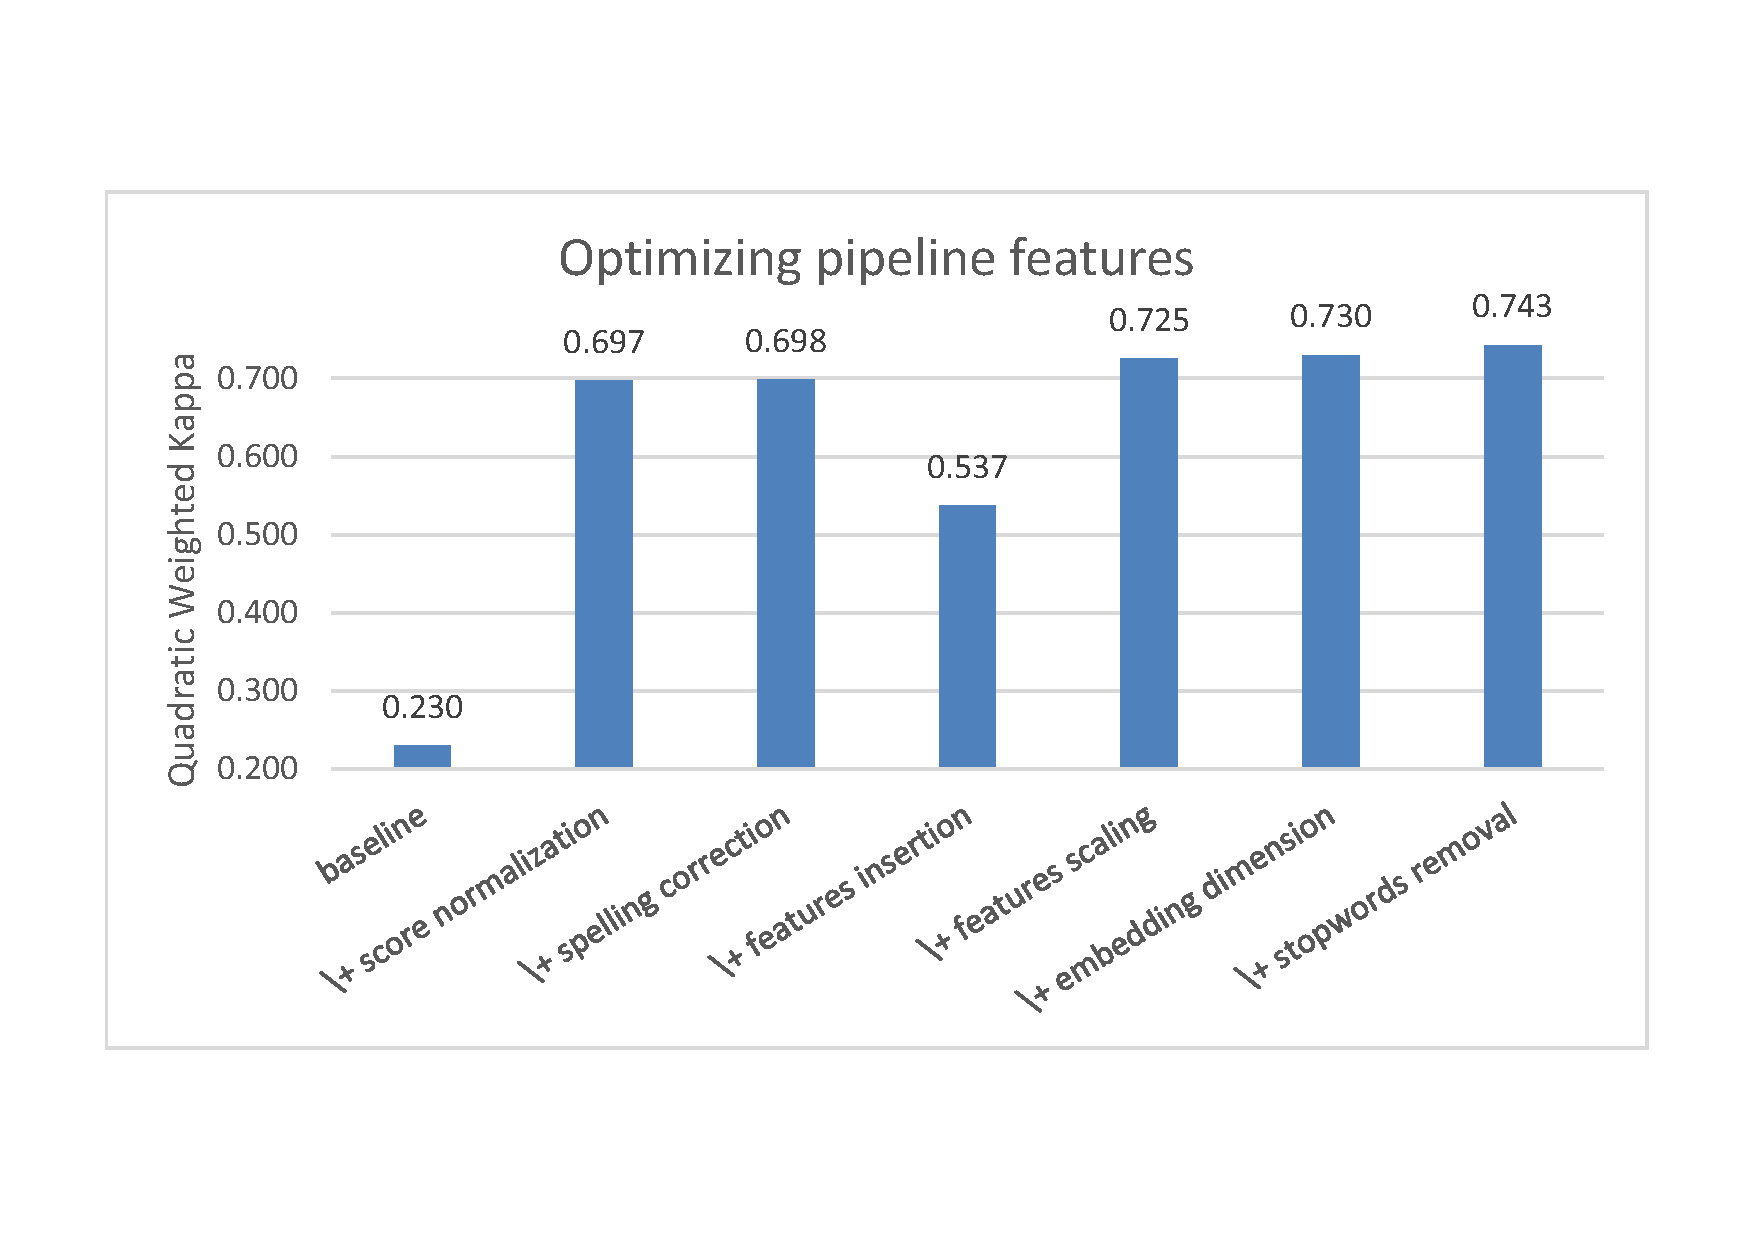
\includegraphics[width=0.85\textwidth]{fig/opt_pip_feat.pdf}
\vspace*{-1.5cm}
\end{center}

\textbf{Hyperparameters tuning} Then we focused on tuning the key learning hyperparameters. For the choice of the learning rate, two values ($0.001$ and $0.01$) led to similar results. We selected $0.01$ because it was slightly better. For the batch size, results indicated that we should select either a small batch size or a very large one. As it speeds up the learning process we decided to go with a rather large batch size ($256$).

\begin{center}
\vspace*{-1.5cm}
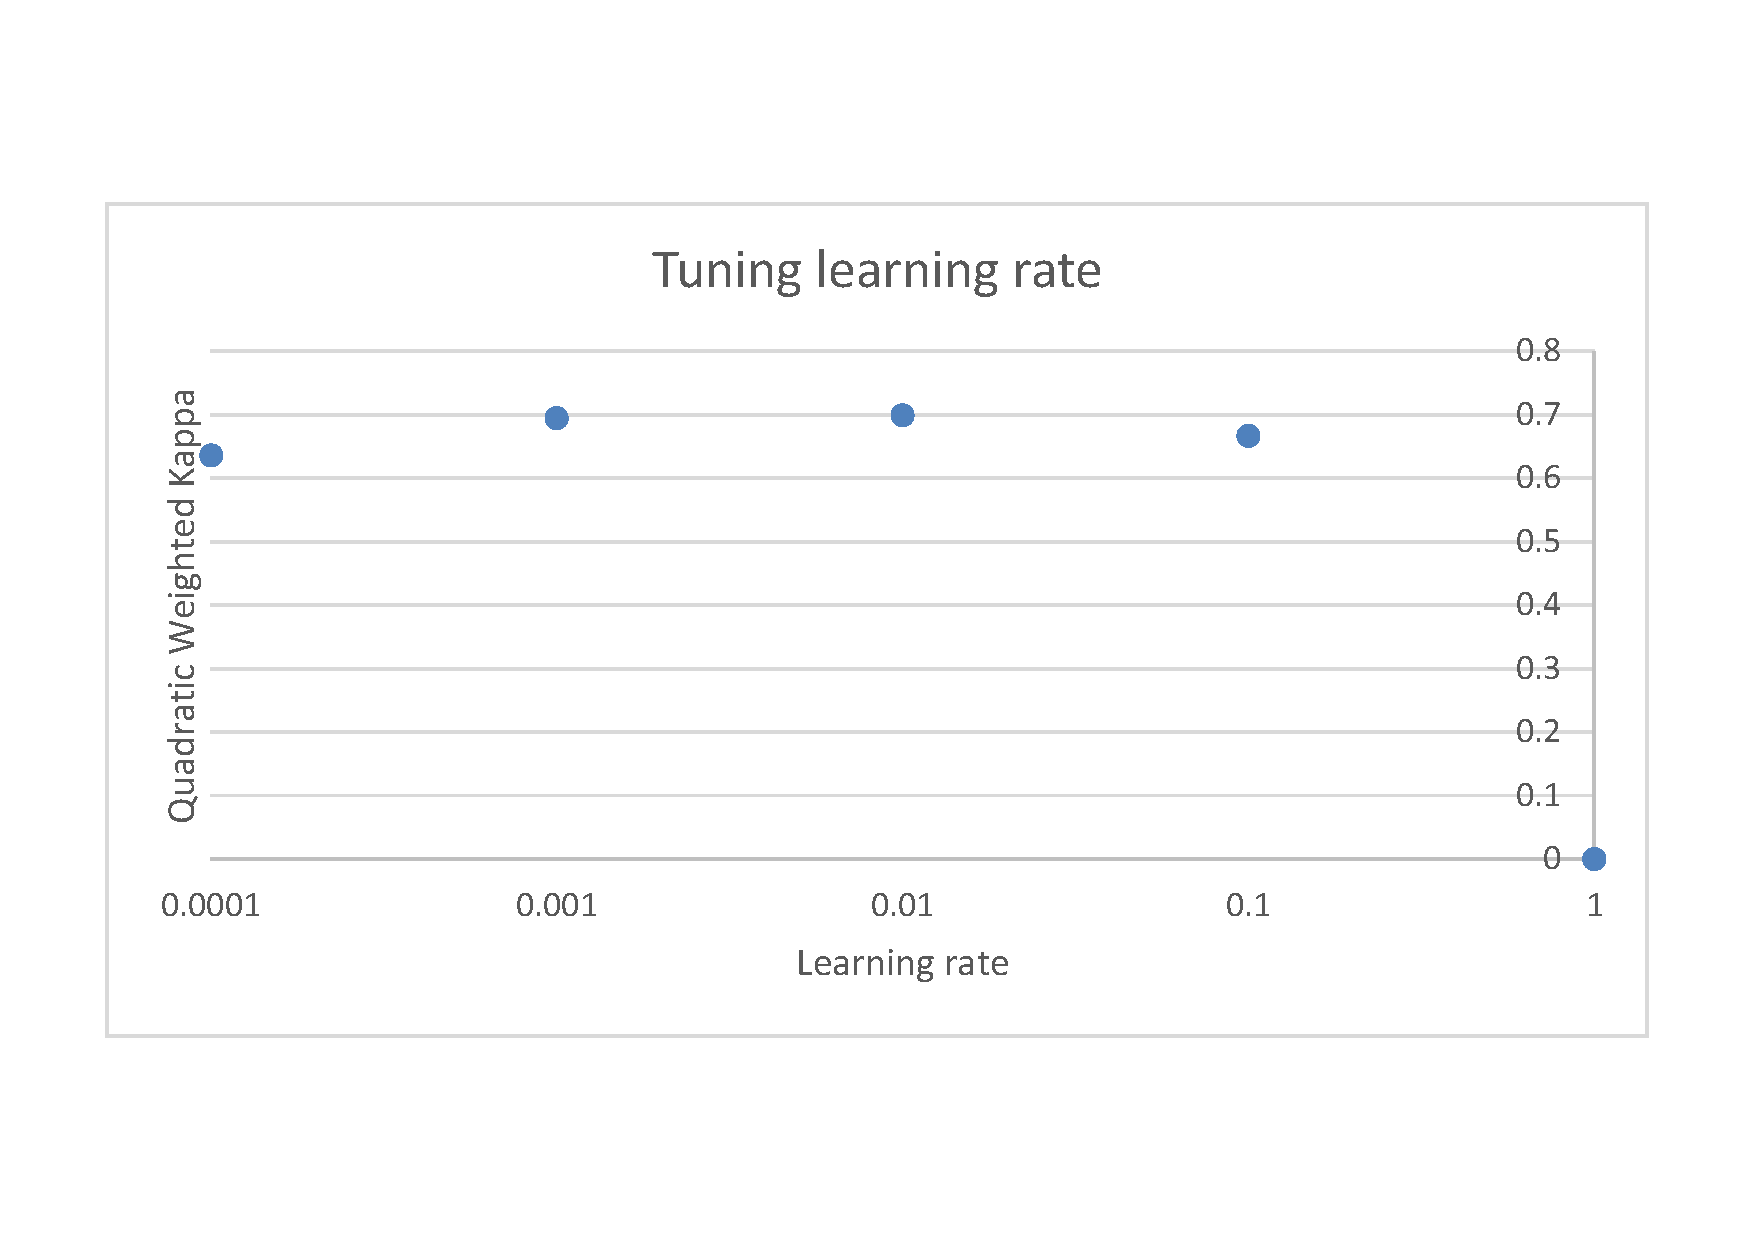
\includegraphics[width=0.85\textwidth]{fig/tune_lr.pdf}
\vspace*{-1.5cm}
\end{center}

\begin{center}
\vspace*{-1.5cm}
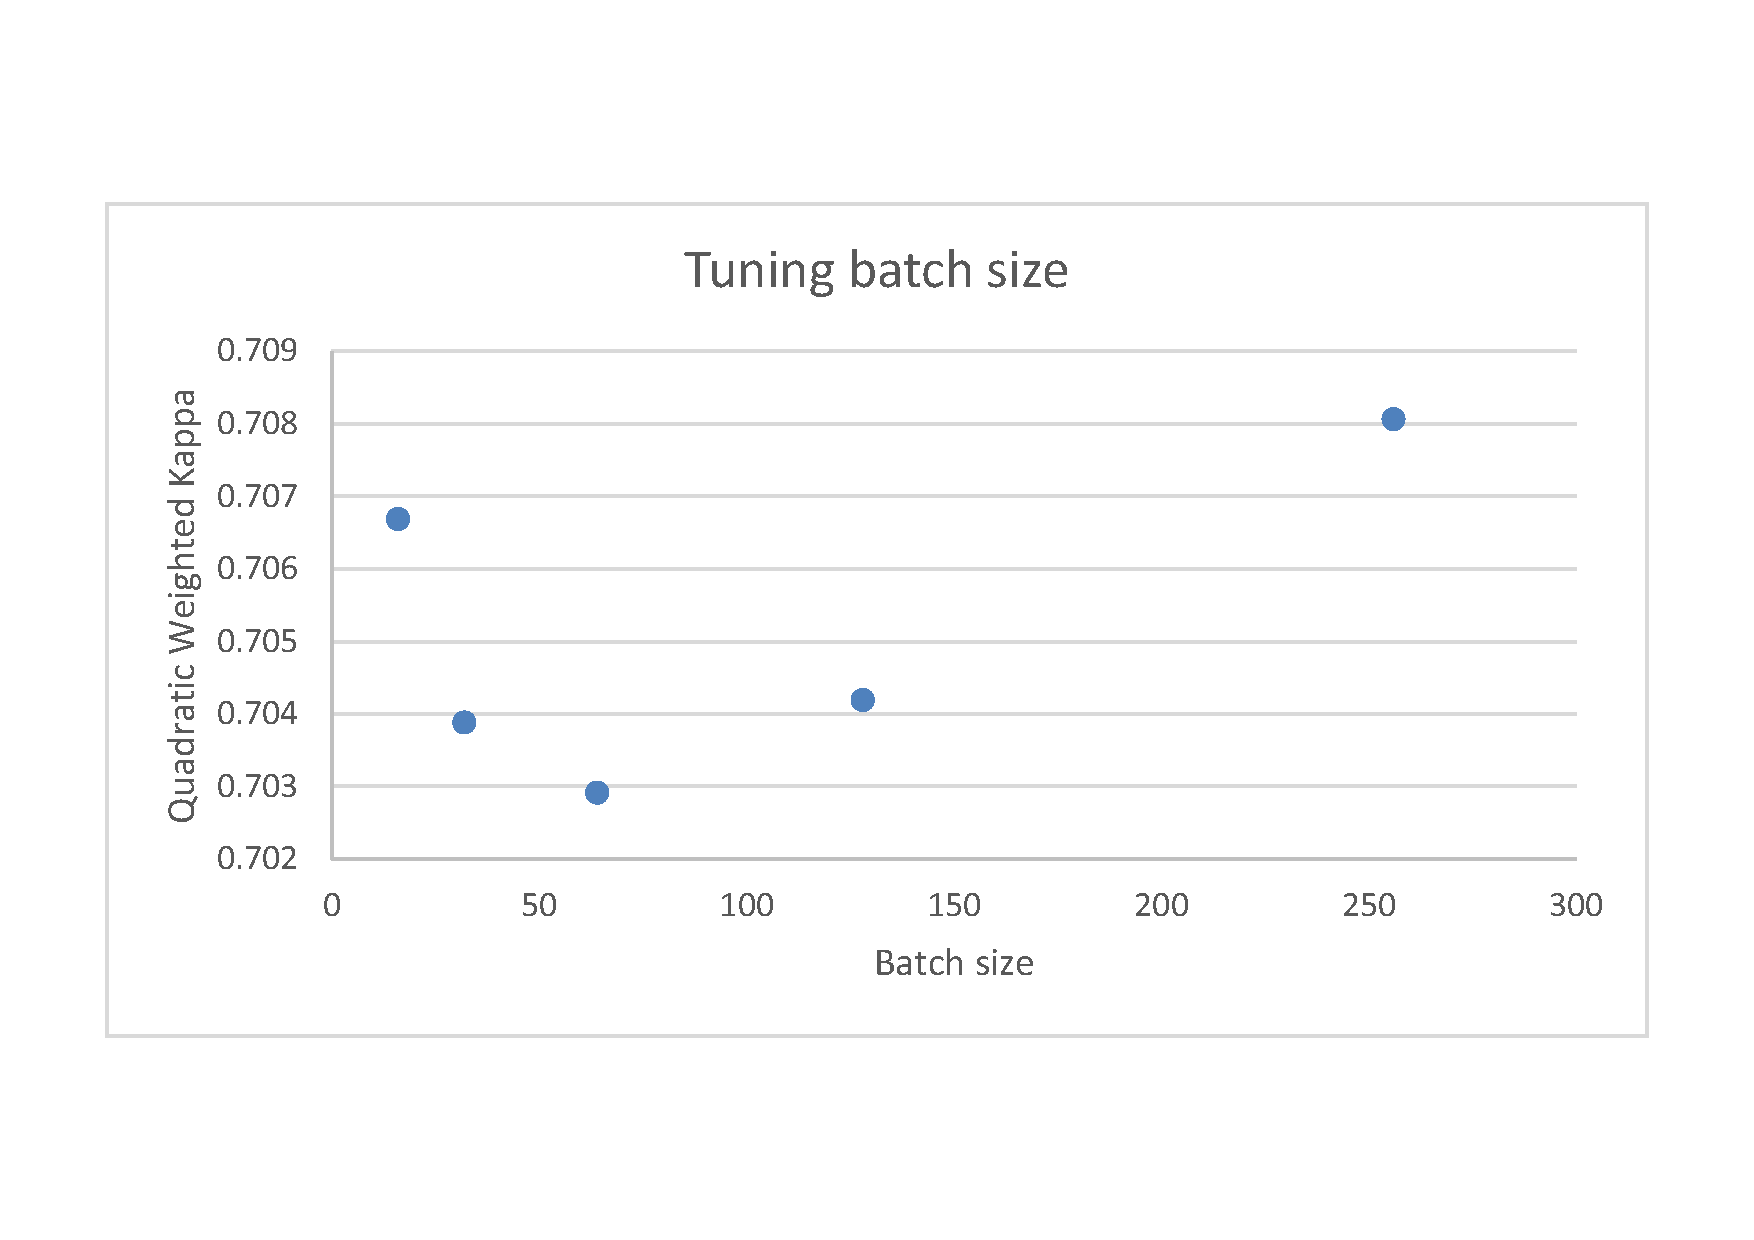
\includegraphics[width=0.85\textwidth]{fig/tune_bs.pdf}
\vspace*{-1.5cm}
\end{center}

\textbf{Dense model optimization} We tried various architecture for the fully connected model. We show the results for different dropout values and number of parameters. The results shown correspond to learning from embedded essays as well as extra-features. We also tried learning solely from extra-features a reached a quadratic weighted kappa value of $0.678$ which is far from the best results we can get when combining embedded essays and extra-features. The best configuration for the dense model is obtained with hidden layers of size $300$ and $128$ and dropout of $0.2$.

\begin{center}
\vspace*{-1.5cm}
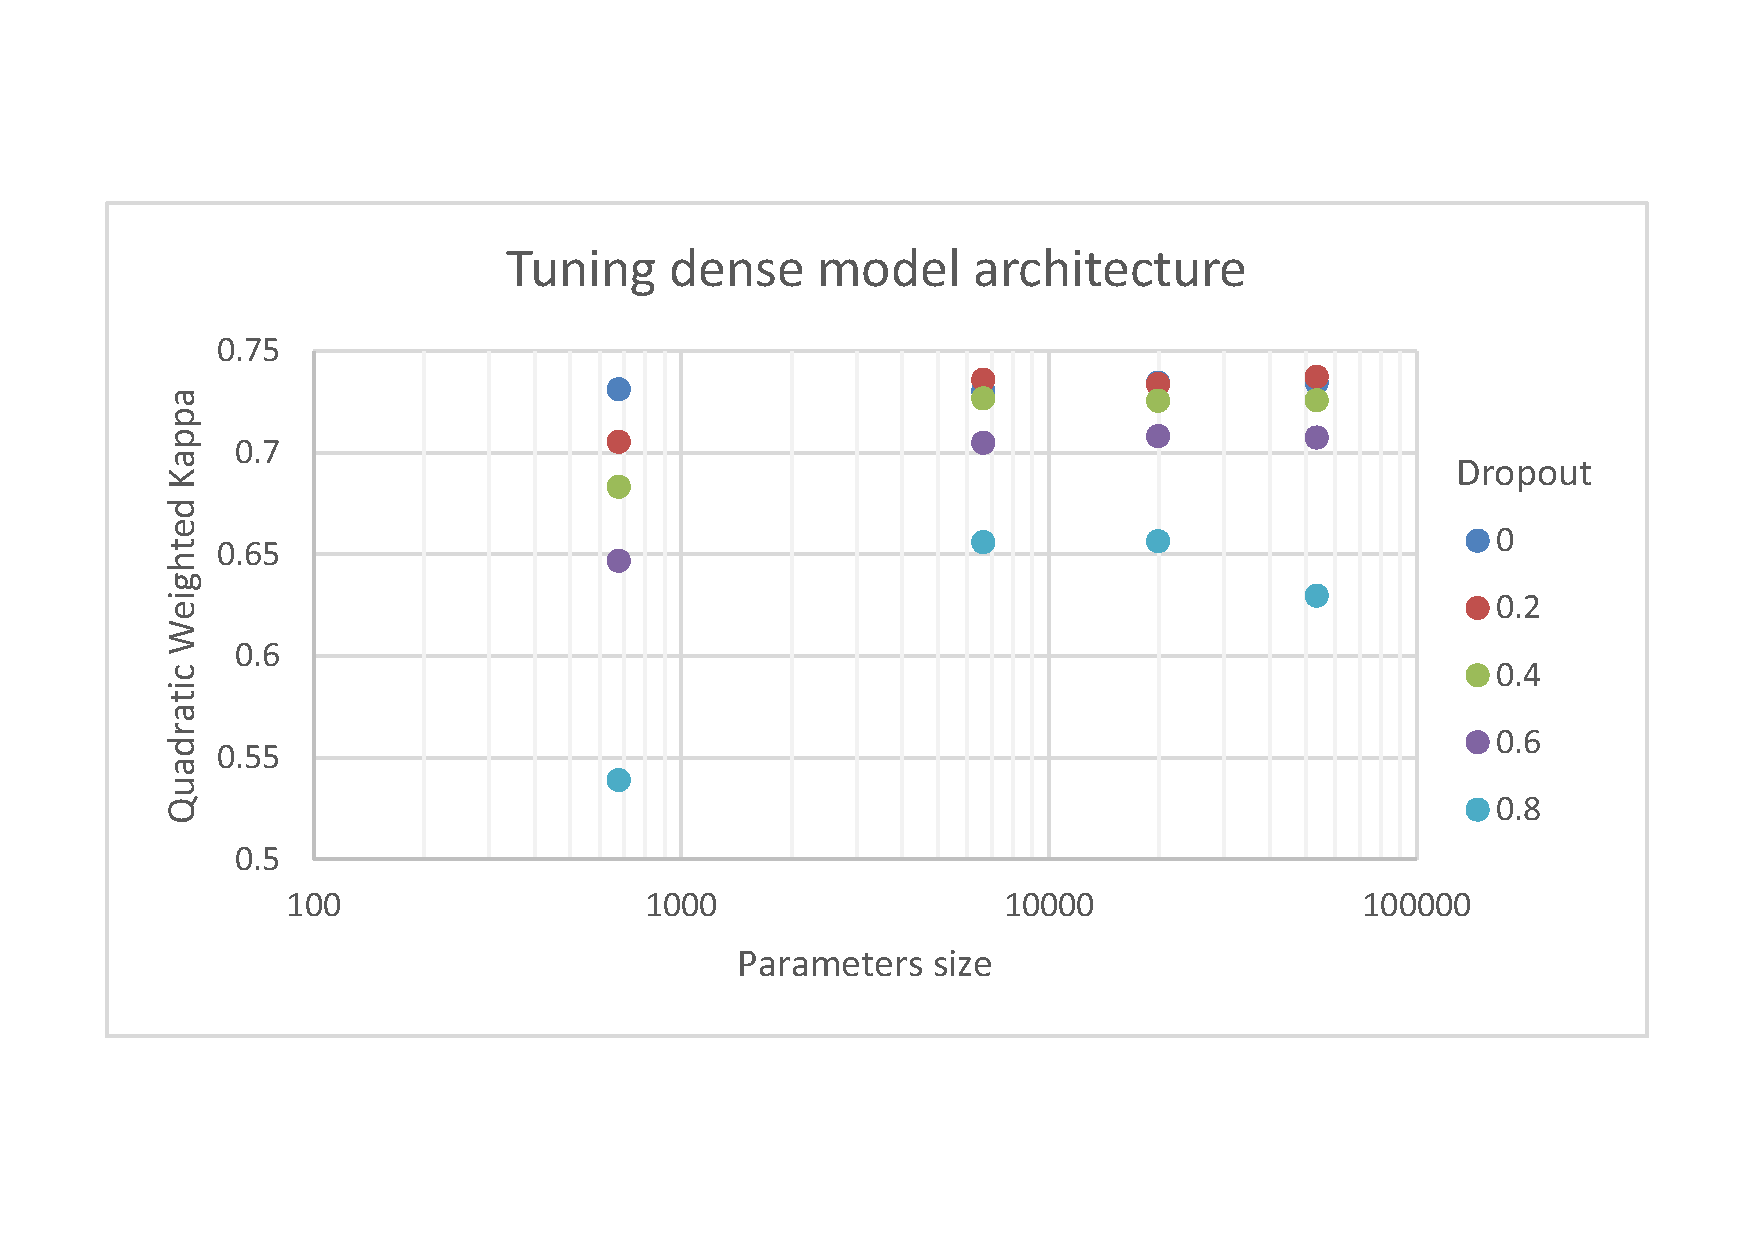
\includegraphics[width=0.85\textwidth]{fig/tune_dense_arch.pdf}
\vspace*{-1.5cm}
\end{center}

\textbf{LSTM model optimization} We conducted similar experiments for our LSTM model. The best LSTM model was obtained with hidden layer size of $100$ for the recurrent units and $16$ for the fully connected part and droupout value of $0.2$. We then tried deeper model architectures by stacking recurrent units on top of each other. Results show that a depth of $4$ is optimal in our case.

\begin{center}
\vspace*{-1.5cm}
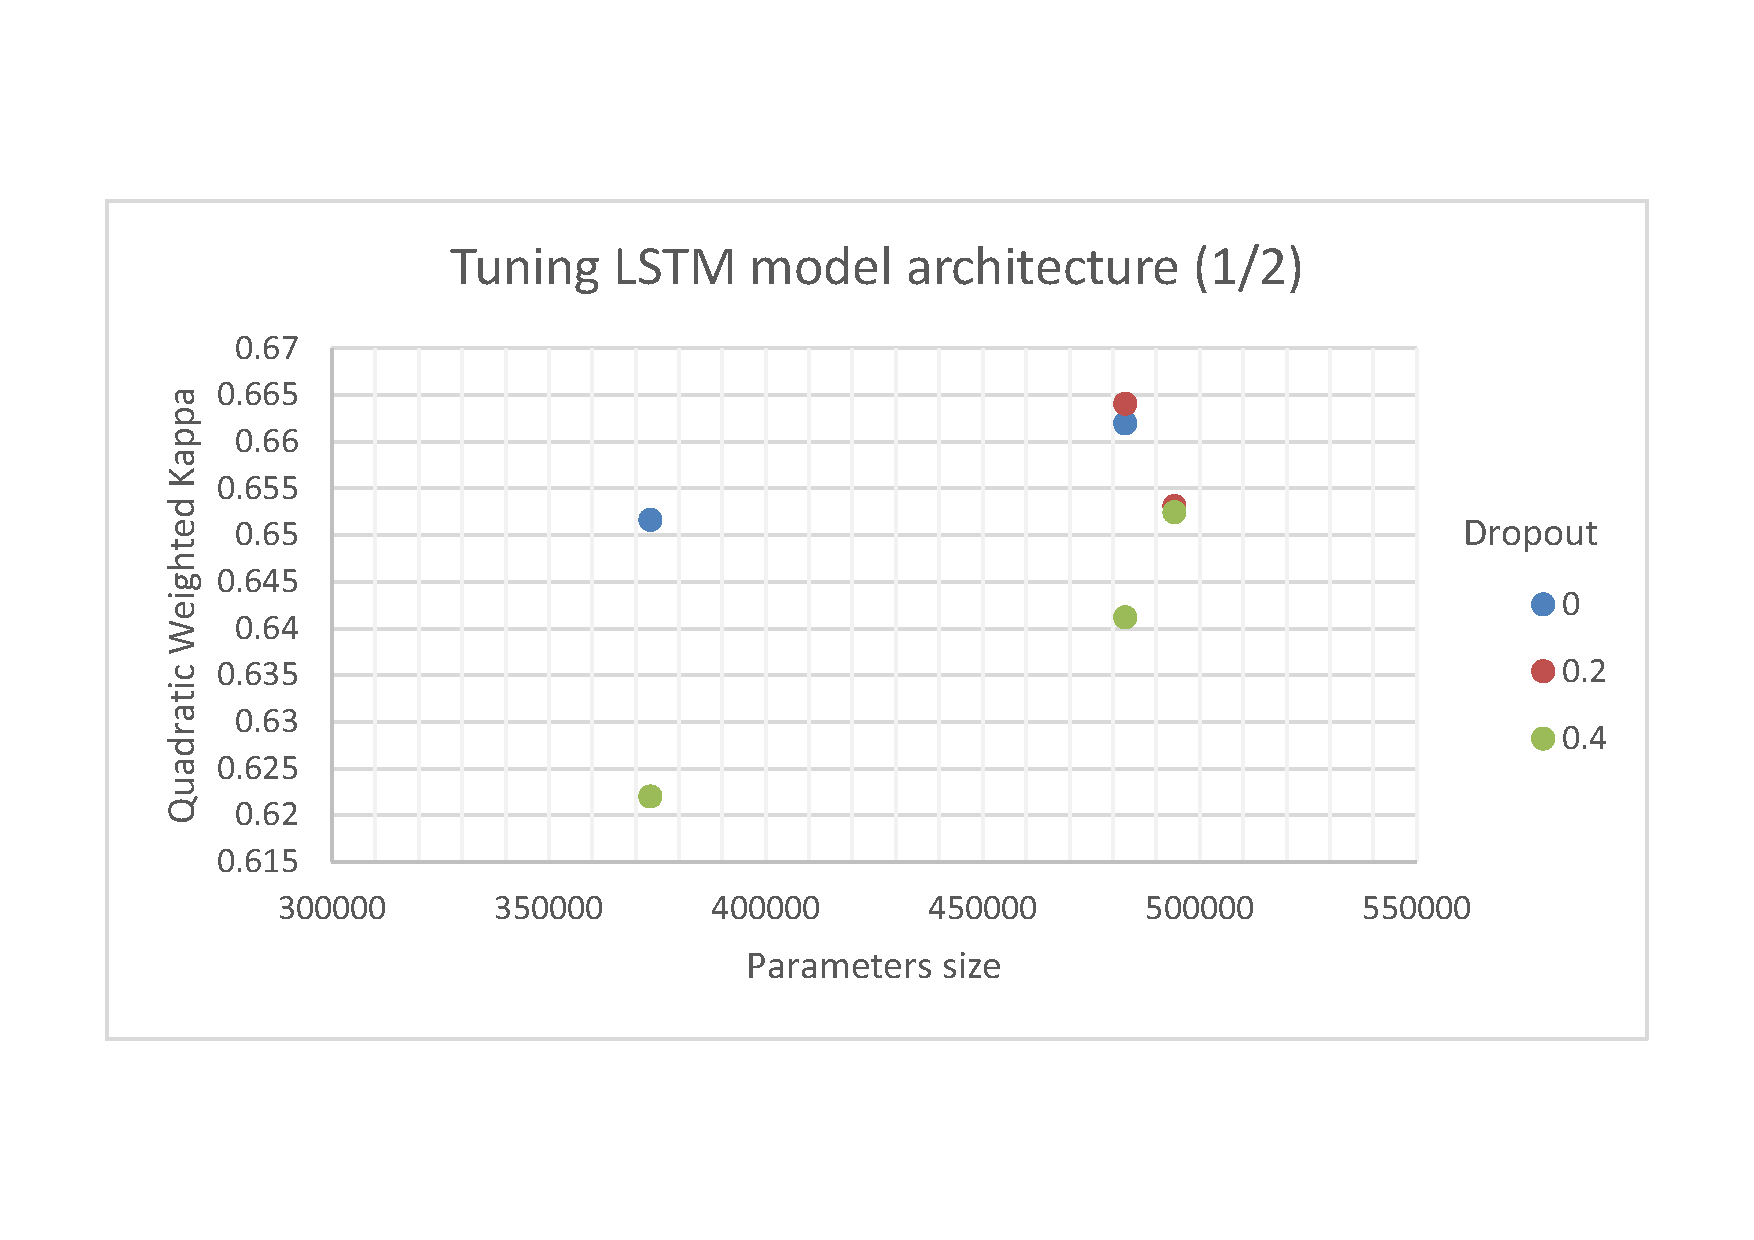
\includegraphics[width=0.85\textwidth]{fig/tune_lstm_arch_1.pdf}
\vspace*{-1.5cm}
\end{center}

\begin{center}
\vspace*{-1.5cm}
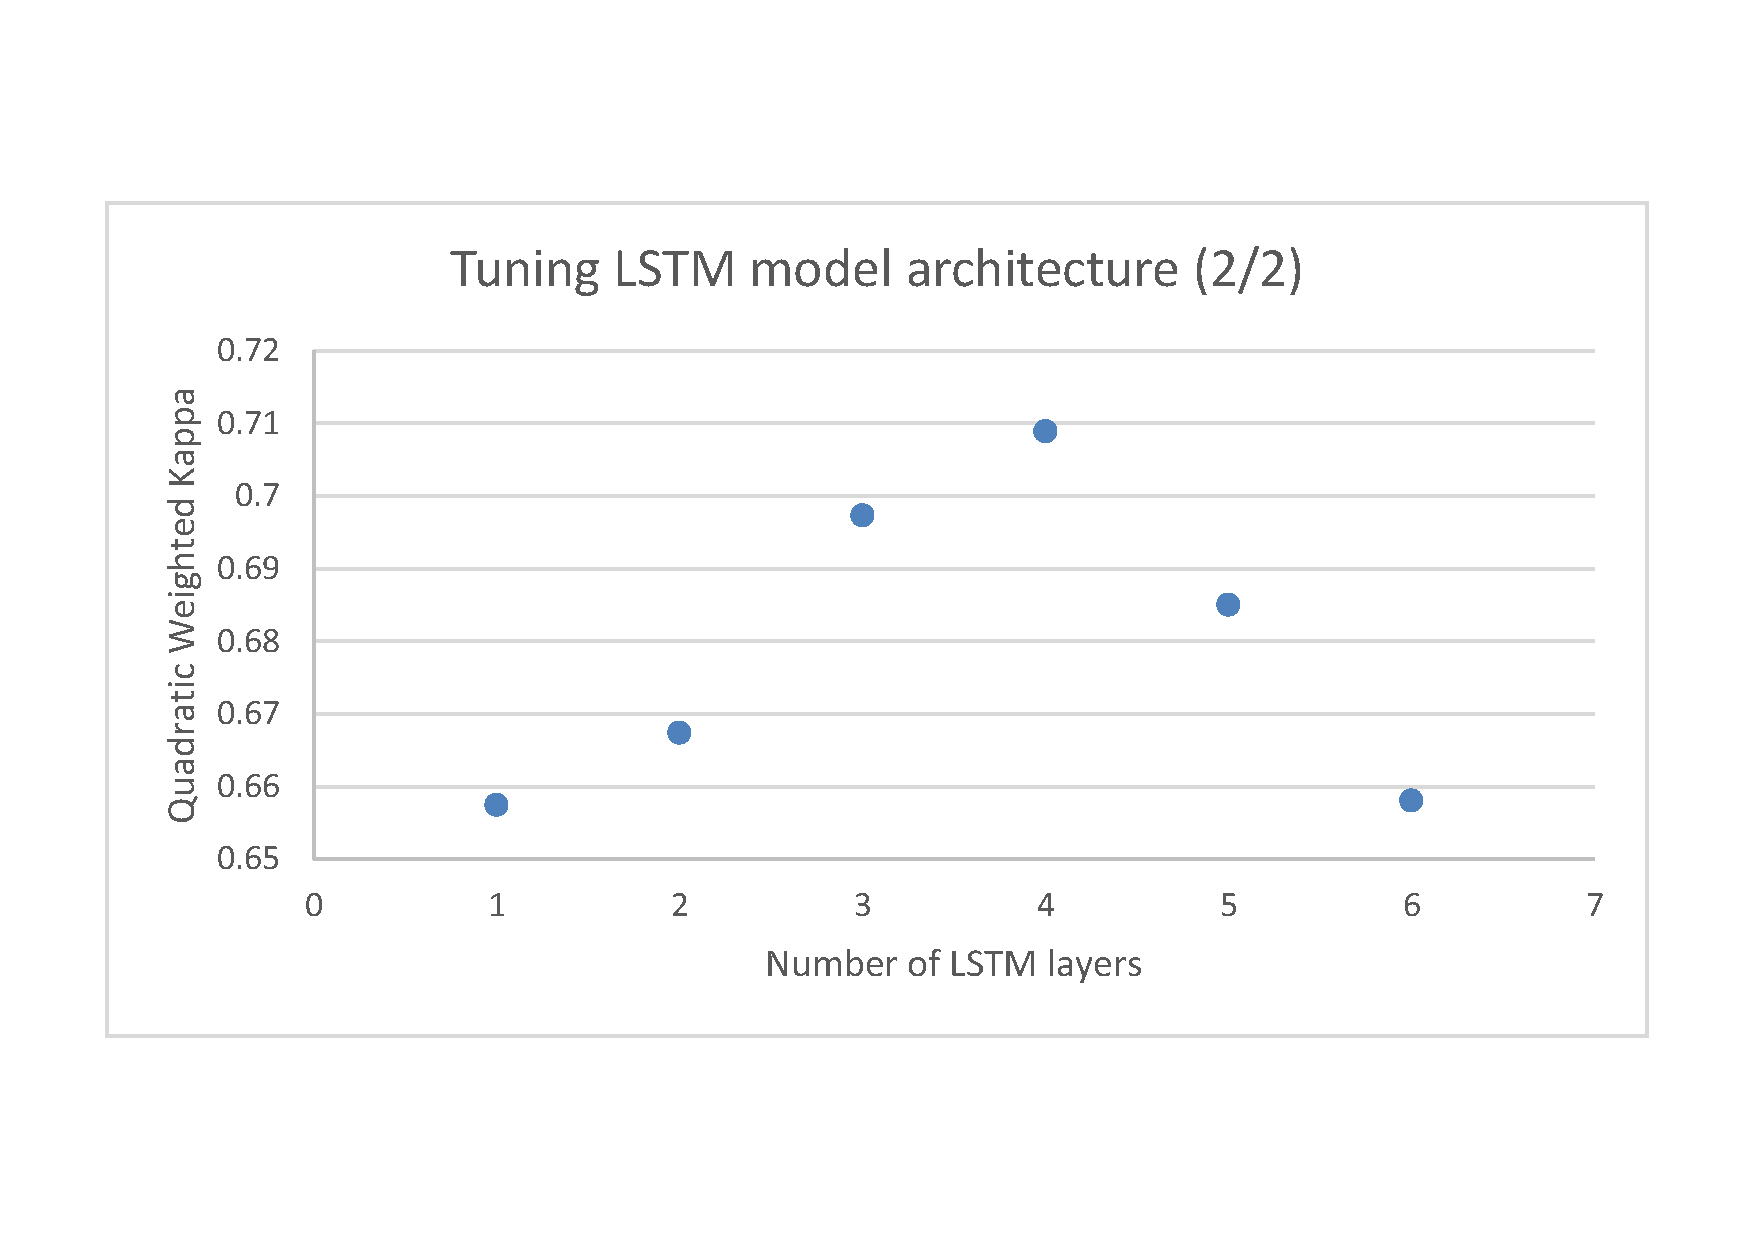
\includegraphics[width=0.85\textwidth]{fig/tune_lstm_arch_2.pdf}
\vspace*{-1.5cm}
\end{center}

\textbf{Joint vs individual models} Multitask models are increasingly popular because achieving a good performance level for one task can help tackling other tasks. However, when we compare the results for our joint model compared to the results of individual models we achieve similar performance. Indeed, the quadratic weighted kappa for the joint model is $0.741$ and $0.744$ when compiling results together for individual models. The small difference is due to the joint model not being very good on the $8$\textsuperscript{th} essay set due to size imbalance between sets. Nevertheless, we prefer to keep the joint model as it is much faster to train and less likely to overfit.

\begin{center}
\vspace*{-1.5cm}
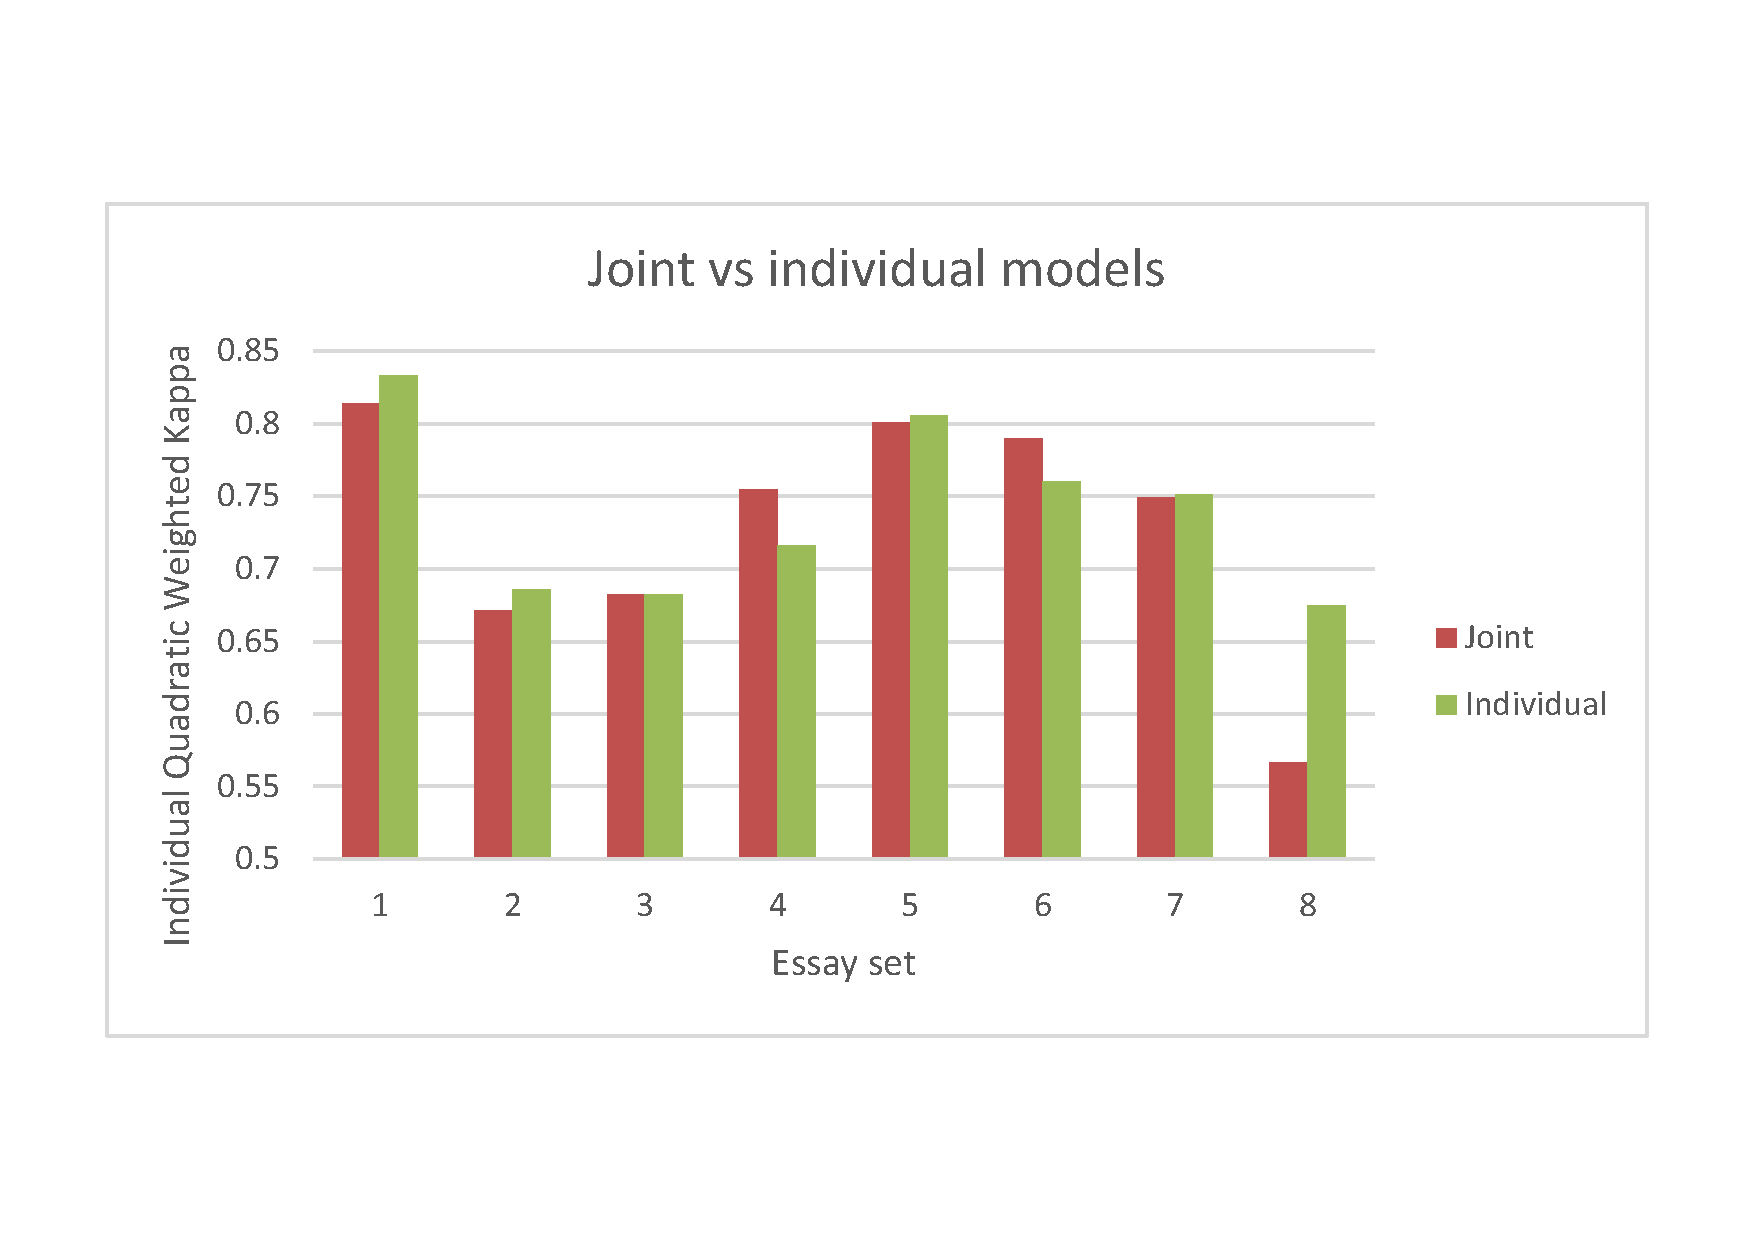
\includegraphics[width=0.85\textwidth]{fig/joint_vs_indiv.pdf}
\vspace*{-1.5cm}
\end{center}

\textbf{Word embeddings comparison} We compare all the proposed word embedding strategies. It turns out that the most successful word embedding strategy is the Word2Vec embedding trained on the essay sentences. We think this is due to specific words and contexts being good indicators for the value of an essay. This strategy leverages the whole corpus thus having task specific knowledge for each of the essay tasks.

\begin{center}
\vspace*{-1.5cm}
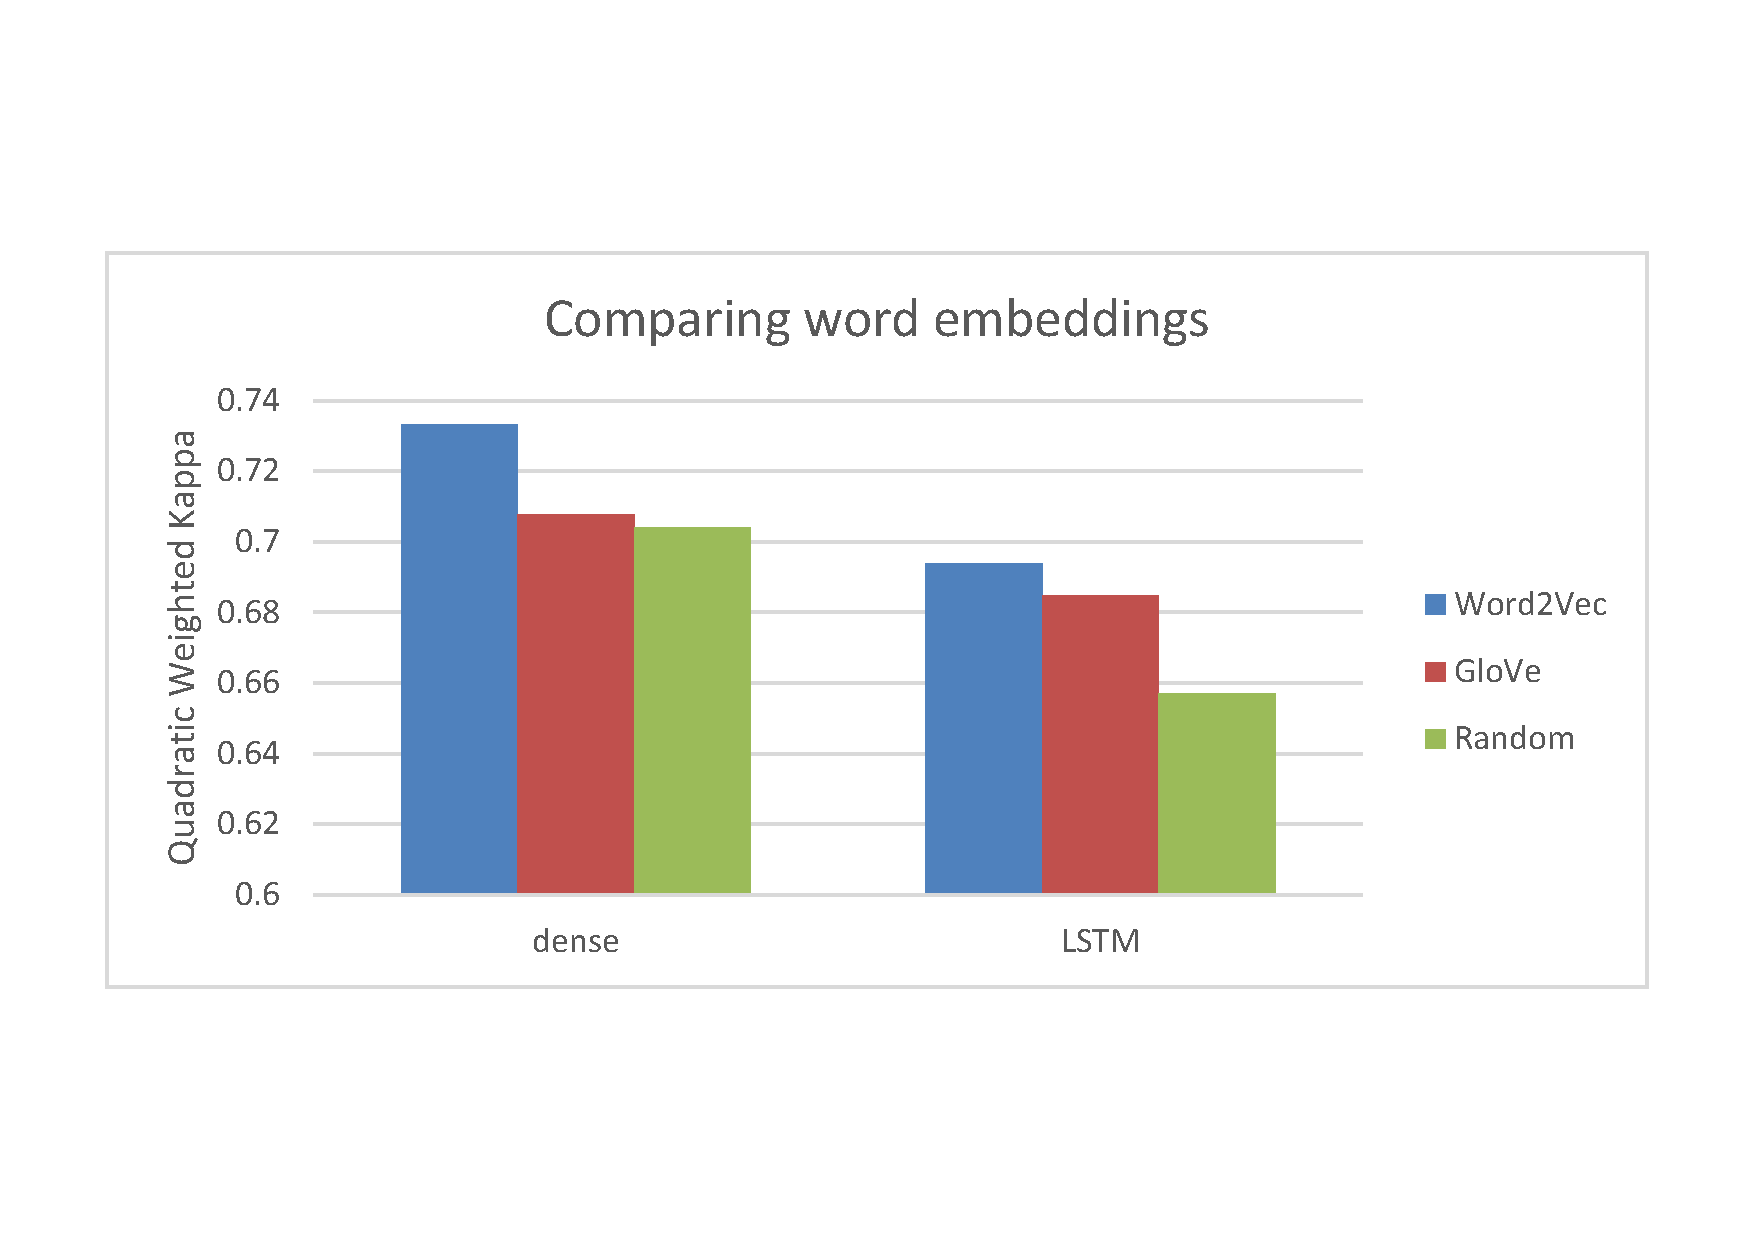
\includegraphics[width=0.85\textwidth]{fig/word_embeddings.pdf}
\vspace*{-1.5cm}
\end{center}

\textbf{Test results} We show the performance of the best model on the test set compared to the performance on the validation set. The individual quadratic weighted kappa are equivalent for all sets except the last one. The reason for this is that the score range is the largest for the 8\textsuperscript{th} set and the kappa metric is expecting identical scores to count true positives. So even if the scores are close the kappa can be low. Moreover the 8\textsuperscript{th} set contains less training samples so it is harder to generalize to unseen essays for this set. All in all, the overall performance is quite satisfying and comparable to other works dedicated to this Kaggle competition.

\begin{center}
\vspace*{-1.5cm}
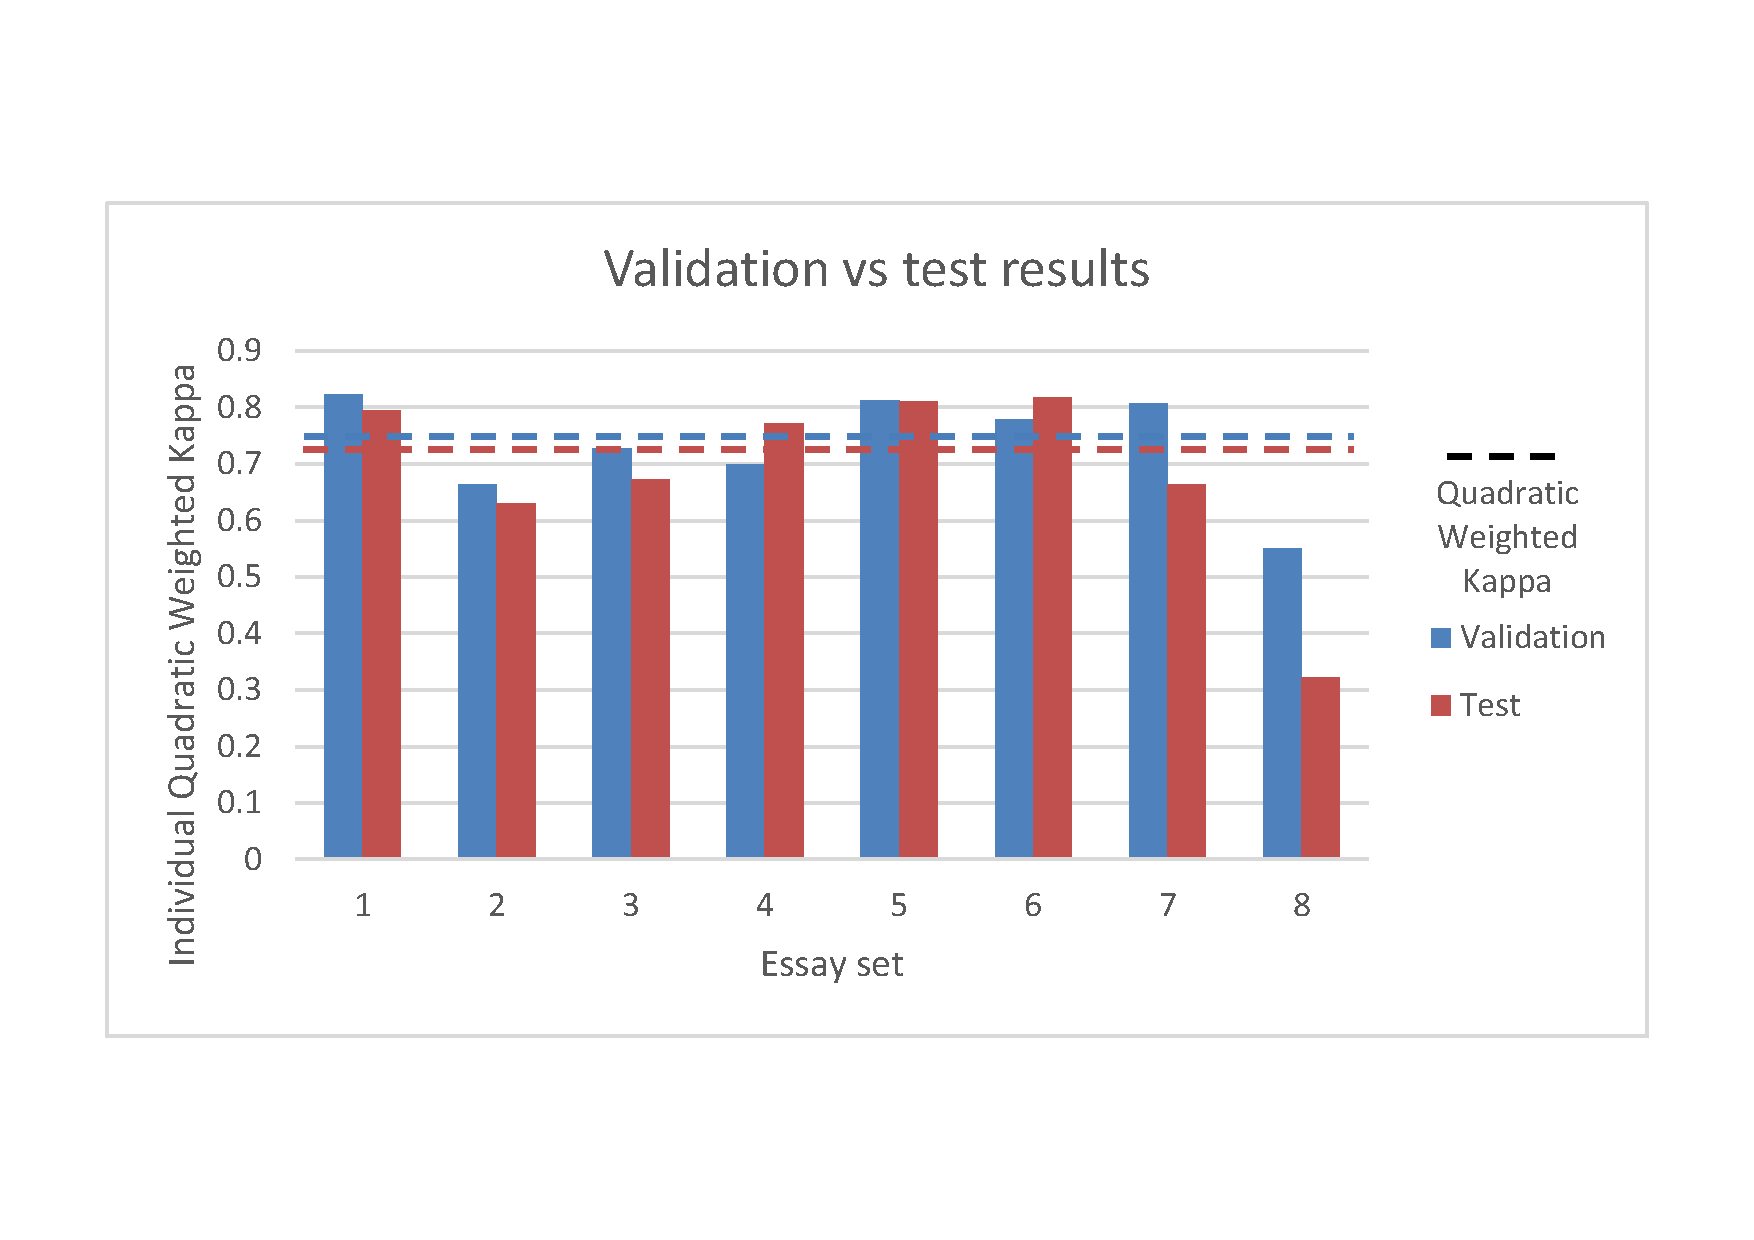
\includegraphics[width=0.85\textwidth]{fig/test.pdf}
\vspace*{-1.5cm}
\end{center}

\TODO{courbes et commentaires pour CNN}

\section{Conclusion}
\TODO{}

\bibliography{ref} 
\bibliographystyle{ieeetr}
\addcontentsline{toc}{section}{References}

\end{document}

